\section{Gestion des enseignements}

Voici les diff{\'e}rents sc{\'e}narios:\\

\section*{Consultant}

\begin{center}
\scalebox{0.7}{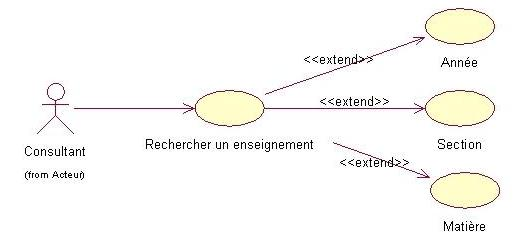
\includegraphics{images/Enseignement_Consultant.jpg}}\\
\end{center}

\begin{tabular}{|p{4cm}|c|p{4cm}|p{5cm}|}
\hline
  Fonction & Priorit{\'e} & Qualit{\'e} & Mesure \\
\hline
Rechercher un enseignement & 3 & Facile et Rapide & Recherche par mots
  cl{\'e}s et efficace.\\
\hline
\end{tabular}

\begin{center}
{\'e}chelle de mesure de la priorit{\'e}:

\scalebox{0.5}{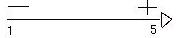
\includegraphics{images/echelle.jpg}}
\end{center}

\begin{itemize}
\item {\bf Rechercher un enseignement :}
	\begin{itemize}
	\item Pr{\'e}-requis : Il doit exister au moins un enseignement
	\item Description : Il selectionne l'option {\it Rechercher un enseignement}.\\
	il saisie au choix l'ann{\'e}e, la section, et la mati{\`e}re. 
	\item Post-requis : Affiche tous les tds et les projets en relation avec l'enseignement sous forme de liste.
	\end{itemize}
\end{itemize}

\section*{Enseignant}

\begin{center}
\scalebox{0.7}{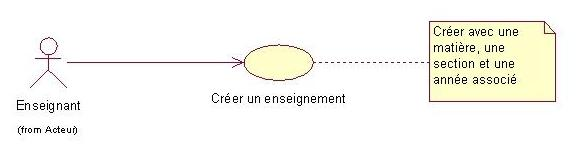
\includegraphics{images/Enseignement_Enseignant.jpg}}\\
\end{center}

\begin{tabular}{|p{4cm}|c|p{4cm}|p{5cm}|}
\hline
  Fonction & Priorit{\'e} & Qualit{\'e} & Mesure \\
\hline
Creer un enseignement & 5 & Facile & Utilisation de menus simples.\\
\hline
\end{tabular}

\begin{center}
{\'e}chelle de mesure de la priorit{\'e}:
\scalebox{0.5}{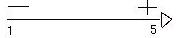
\includegraphics{images/echelle.jpg}}
\end{center}

\begin{itemize}
\item {\bf Cr�er un enseignement :}
	\begin{itemize}
	\item Pr{\'e}-requis : Etre log{\'e}, avoir des mati{\`e}res et des sections d{\'e}j{\`a} existantes.
	\item Description : Il s'identifie avec son login et son mot de passe. \\
	Il saisie une ann{\'e}e et s{\'e}lectionne successivement une section et une mati{\`e}re.\\
	Il d{\'e}signe le nom du nouvel enseignement qu'il veut cr{\'e}er. Il valide ses choix.
	\item Post-requis : Un nouvel enseignement est cr{\'e}{\'e}.
	\end{itemize}
\end{itemize}


\section*{Administrateur}

\begin{center}
\scalebox{0.7}{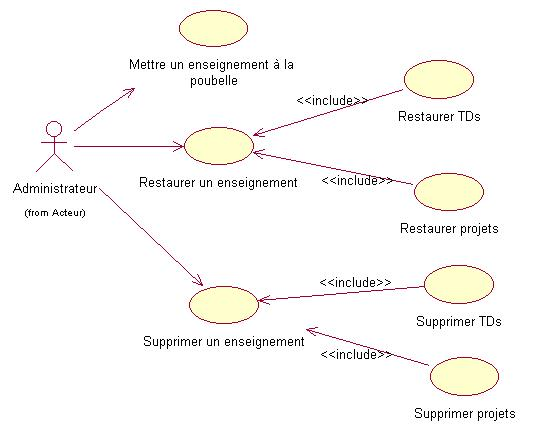
\includegraphics{images/Enseignement_Administrateur.jpg}}\\
\end{center}

\begin{tabular}{|p{4cm}|c|p{4cm}|p{5cm}|}
\hline
  Fonction & Priorit{\'e} & Qualit{\'e} & Mesure \\
\hline
D{\'e}placer vers la corbeille un enseignement & 4 & Fiable et S{\^u}r & Ne pas supprimer un autre
  ensignement que celui s{\'e}lectionn{\'e}. Les devoirs de l'enseignement
  sont archiv{\'e}s. \\
\hline
Suppression totale de l'enseignement & 3 & Rapide et s�r  & La suppresion d'un enseignement dans la corbeille doit �tre rapide\\
\hline
Restaurer l'enseignement & 4 & S�r & Un enseignement dans la corbeille doit pouvoir �tre restaurer sans aucune perte d'informations.\\
\hline
\end{tabular}

\begin{center}
{\'e}chelle de mesure de la priorit{\'e}:

\scalebox{0.5}{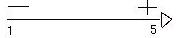
\includegraphics{images/echelle.jpg}}
\end{center}

\begin{itemize}
\item {\bf D{\'e}placer vers la corbeille un enseignement :}
	\begin{itemize}
	\item Pr{\'e}-requis : Etre log{\'e}. Il doit exister au moins un TDs ou projets.
	\item Description : IL d{\'e}place les TDs ou les projets vers la corbeille.\\
	 C'est en fait une suppression partiel car ils peuvent {\^e}tre restaur{\'e} tant que l'administrateur ne l'a pas supprim{\'e} totalement.
	\item Post-requis : Le Td ou le projet d{\'e}plac{\'e} n'est plus dans le liste des tds ou des projets.\\
	\end{itemize}

\item {\bf Suppression de l'enseignement:}
	\begin{itemize}
	\item Pr{\'e}-requis : Etre log{\'e}. Il doit exister au moins un enseignement dans la corbeille.
	\item Description : Il selectionne l'enseignement qui veut supprimer et valide la suppresion.
	\item Post-requis : L'enseignement est compl{\`e}tement supprim{\'e}. Il est irr{\'e}cup{\'e}rable.\\
	\end{itemize}

\item {\bf Restaurer l'enseignement:}
	\begin{itemize}
	\item Pr{\'e}-requis : Etre log{\'e}. Il doit exister au moins un enseignement dans la corbeille.
	\item Description : Il selectionne l'enseignement qui veut restaurer et valide la restauration.
	\item Post-requis : L'enseignement est restaur{\'e} � l'endroit ou il {\'e}tait avant suppression avec les options qu'il avait avant suppression.\\
	\end{itemize}
\end{itemize}